\documentclass[aspectratio=43]{beamer}
\usepackage[english]{babel}
\usepackage{amsthm}
\usepackage{calligra}
\usepackage{csquotes}
\usepackage[thicklines]{cancel}
\usepackage{tcolorbox}
\usepackage{pstricks}
\usepackage[utf8]{inputenc}
\usepackage[backend=biber, bibstyle=nature, sorting=nty, citestyle=numeric-comp]{biblatex}
    \addbibresource{bib.bib}


\def\rc{\scriptr}
\def\brc{\boldscriptr}
\def\hrc{\hat\brc}

\useoutertheme{infolines}
\useinnertheme{rectangles}
\usefonttheme{professionalfonts}


\definecolor{orange}{HTML}{f28165}
\definecolor{gray}{HTML}{303030}
\definecolor{yellow}{HTML}{f0be52}
\definecolor{lightorange}{HTML}{f19e58}

\renewcommand{\CancelColor}{\color{orange}}

\makeatletter
\newcommand{\mybox}[1]{%
  \setbox0=\hbox{#1}%
  \setlength{\@tempdima}{\dimexpr\wd0+13pt}%
  \begin{tcolorbox}[colback=orange,colframe=orange,boxrule=0.5pt,arc=4pt,
      left=6pt,right=6pt,top=6pt,bottom=6pt,boxsep=0pt,width=\@tempdima]
    \textcolor{white}{#1}
  \end{tcolorbox}
}
\makeatother

\usecolortheme[named=orange]{structure}
\usecolortheme{sidebartab}
\usecolortheme{orchid}
\usecolortheme{whale}
\setbeamercolor{alerted text}{fg=yellow}
\setbeamercolor{block title alerted}{bg=alerted text.fg!90!black}
\setbeamercolor{block title example}{bg=lightorange!60!black}
\setbeamercolor{background canvas}{bg=gray}
\setbeamercolor{normal text}{bg=gray,fg=white}

\setbeamertemplate{footline}
        {
      \vskip0pt%

      \leavevmode%
      \hbox{%
      \begin{beamercolorbox}[wd=.333333\paperwidth,ht=2.25ex,dp=1ex,center]{author in head/foot}%
        \usebeamerfont{author in head/foot}\insertshortauthor
      \end{beamercolorbox}%
      \begin{beamercolorbox}[wd=.333333\paperwidth,ht=2.25ex,dp=1ex,center]{title in head/foot}%
        \usebeamerfont{title in head/foot}\insertshorttitle
      \end{beamercolorbox}%
      \begin{beamercolorbox}[wd=.333333\paperwidth,ht=2.25ex,dp=1ex,center]{date in head/foot}%
        \usebeamerfont{date in head/foot}\insertshortinstitute{}

      \end{beamercolorbox}}%
    }


\setbeamertemplate{blocks}[rectangle]

\setbeamertemplate{frametitle continuation}{}
\setbeamercovered{dynamic}

\setbeamertemplate{section page}
{
	\begin{centering}
		\begin{beamercolorbox}[sep=27pt,center]{part title}
			\usebeamerfont{section title}\insertsection\par
			\usebeamerfont{subsection title}\insertsubsection\par
		\end{beamercolorbox}
	\end{centering}
}


\newcommand{\hlight}[1]{\colorbox{violet!50}{#1}}
\newcommand{\hlighta}[1]{\colorbox{red!50}{#1}}
\title{Analizador Léxico}
\subtitle{Proyecto 1}
\author[Jose P. Fernández, Roberto Vidal]{
    Jose Pablo Fernández Cubillo%
    \\%
    Roberto Vidal Patiño%
}
\institute[Tecnológico de Costa Rica]{
    Tecnológico de Costa Rica%
    \\%
    Compiladores e Intérpretes%
}
\date{I Semestre, 2021}

\begin{document}
    
    \frame{\titlepage}

    \begin{frame}{Preprocesador}
            El preprocesador es basado en el que se usa para el lenguaje c. Cuenta con 4 fases. \\
            \begin{enumerate}
                \item Remplazo de digrafos y trigrafos.
                \begin{enumerate}
                    \item Digrafos: \textless : :\textgreater, \textless \%, \% \textgreater \% :
                    \item Trigrafos empiezan con ??.
                \end{enumerate}
                \item Empalmado de líneas (si una línea termina con \ se omite el salto de línea concatenandola como si fuera la misma).
                \item Remplazo de comentarios y divide tokens por un caracter de separación.
                \item Expansión de macros.
                \begin{enumerate}
                    \item También implementamos los que son con parámetros.
                \end{enumerate}
            \end{enumerate}
    \end{frame}

    \begin{frame}{Tabla de dígrafos}
        \begin{table}
            \begin{tabular}{c | c}
            Dígrafo & Equivalencia \\
            \hline \hline
                \textless : & [ \\
                :\textgreater & ] \\
                \textless \% & \{ \\
                \% \textgreater & \} \\
                \% : & \# 
            \end{tabular}
            \caption{Tabla de dígrafos}
        \end{table}

    \end{frame}

    \begin{frame}{Tabla de trígrafos}
        \begin{table}
            \begin{tabular}{c | c}
            trígrafo & Equivalencia \\
            \hline \hline
                ??= & \# \\
                ??/ & \textbackslash \\
                ??' & \^{} \\
                ??( & [ \\
                ??) & ] \\
                ??! & \textbar \\
                ??\textless & \{ \\
                ??\textgreater & \} \\
                ??\textendash & \~{}
            \end{tabular}
            \caption{Tabla de trígrafos}
        \end{table}

    \end{frame}
    
    \begin{frame}{Scanning y Herramienta Flex}
            El proceso de scanning consiste en tomar el código fuente, pasarlo por el preprocesador y luego el archivo generado por el preprocesador es el que se mete en el scanner. \\
            \begin{figure}[h]
                \centerline{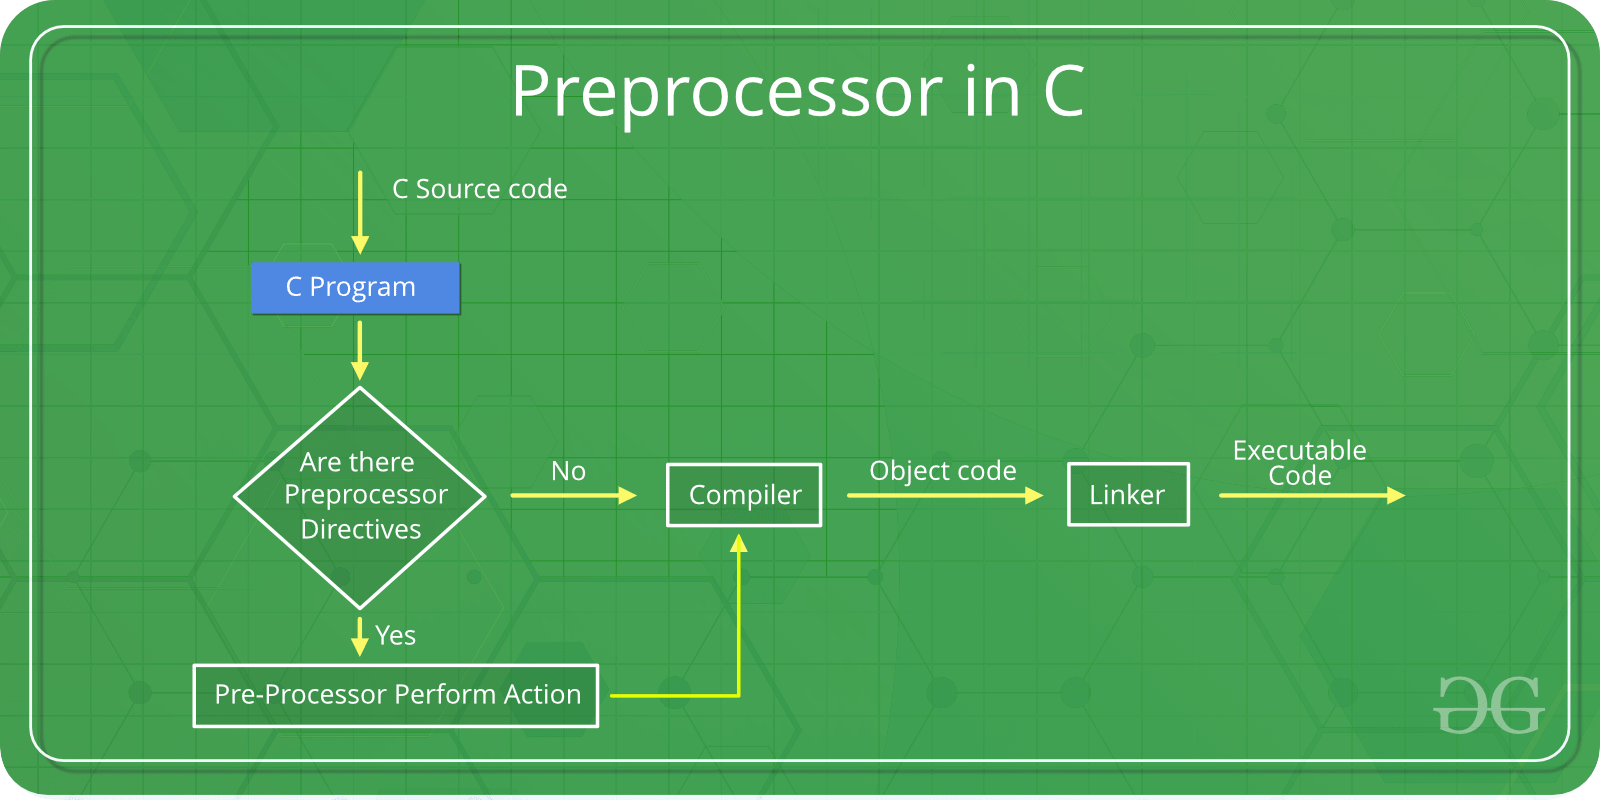
\includegraphics[scale=.15]{preprocessor.png}}
            \end{figure}
    \end{frame}
    
    \begin{frame}{Scanning y Herramienta Flex}
        El uso de la herramienta flex es relativamente sencillo. Primero se debe definir los diferentes tipos de tokens y se coloca en un archivo header, desde flex se puede importar este archivo. Después, se pueden definir algunas expresiones regulares si se necesitan para identificar algún tipo de token. Luego, se coloca la expresión regular o el propio string y el código del token que debe retornar. Generalmente se usa junto a Bison, el cual sería el parser, pero en este caso como solo es el scanner, se utilizó solo flex. \\
        \begin{figure}[h]
            \centerline{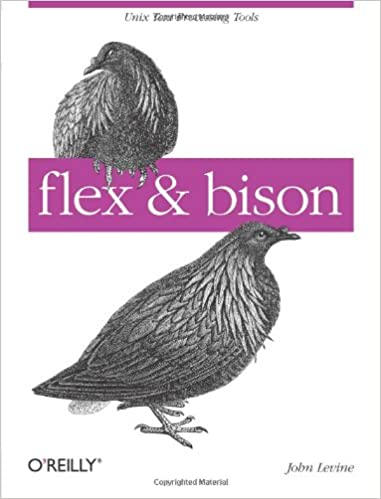
\includegraphics[scale=.20]{flex.jpg}}
        \end{figure}
    \end{frame}

    \section{Programa Fuente} 

 	\frame{\sectionpage} 

\begin{frame}{Formato de tokens} 
		\begin{enumerate} 
			 \item {\textcolor[HTML]{162511}{\colorbox[HTML]{5BF62A}{\fontfamily{lmdh} \selectfont 
				Palabras Reservadas% 
			}}} 
			\item {\textcolor[HTML]{290B26}{\colorbox[HTML]{9F7BBD}{\fontfamily{cmtt}\selectfont 
				Operadores%
			}}} 
			\item {\textcolor[HTML]{B5B5B5}{\colorbox[HTML]{161616}{\fontfamily{cmss}\selectfont 
				String% 
			}}} 
			\item {\textcolor[HTML]{2A1200}{\colorbox[HTML]{FFA562}{\fontfamily{pcr}\selectfont 
				Constantes%
			}}} 
			\item {\textcolor[HTML]{FFF8A0}{\colorbox[HTML]{413C00}{\fontfamily{qag}\selectfont 
				Caracteres Especiales% 
			}}} 
			\item {\textcolor[HTML]{84A8FA}{\colorbox[HTML]{15006A}{\fontfamily{ptm}\selectfont 
				Identificadores% 
			}}} 
			\item {\textcolor[HTML]{FF0000}{\colorbox[HTML]{300707}{\fontfamily{ppl}\selectfont 
				Errores Léxicos% 
			}}} 
		\end{enumerate} 
	\end{frame} 

	\begin{frame}[allowframebreaks, noframenumbering]{Programa Fuente}
		 \textcolor[HTML]{162511}{\colorbox[HTML]{5BF62A}{\fontfamily{lmdh}\selectfont void}} \textcolor[HTML]{84A8FA}{\colorbox[HTML]{15006A}{\fontfamily{ptm}\selectfont printf}} \textcolor[HTML]{FFF8A0}{\colorbox[HTML]{413C00}{\fontfamily{qag}\selectfont (}} \textcolor[HTML]{162511}{\colorbox[HTML]{5BF62A}{\fontfamily{lmdh}\selectfont char}} \textcolor[HTML]{84A8FA}{\colorbox[HTML]{15006A}{\fontfamily{ptm}\selectfont p}} \textcolor[HTML]{FFF8A0}{\colorbox[HTML]{413C00}{\fontfamily{qag}\selectfont [}} \textcolor[HTML]{FFF8A0}{\colorbox[HTML]{413C00}{\fontfamily{qag}\selectfont ]}} \textcolor[HTML]{FFF8A0}{\colorbox[HTML]{413C00}{\fontfamily{qag}\selectfont ,}} \textcolor[HTML]{FFF8A0}{\colorbox[HTML]{413C00}{\fontfamily{qag}\selectfont .}} \textcolor[HTML]{FFF8A0}{\colorbox[HTML]{413C00}{\fontfamily{qag}\selectfont .}} \textcolor[HTML]{FFF8A0}{\colorbox[HTML]{413C00}{\fontfamily{qag}\selectfont .}} \textcolor[HTML]{FFF8A0}{\colorbox[HTML]{413C00}{\fontfamily{qag}\selectfont )}} \textcolor[HTML]{FFF8A0}{\colorbox[HTML]{413C00}{\fontfamily{qag}\selectfont ;}} \newline 
		 \textcolor[HTML]{162511}{\colorbox[HTML]{5BF62A}{\fontfamily{lmdh}\selectfont void}} \textcolor[HTML]{84A8FA}{\colorbox[HTML]{15006A}{\fontfamily{ptm}\selectfont scanf}} \textcolor[HTML]{FFF8A0}{\colorbox[HTML]{413C00}{\fontfamily{qag}\selectfont (}} \textcolor[HTML]{162511}{\colorbox[HTML]{5BF62A}{\fontfamily{lmdh}\selectfont char}} \textcolor[HTML]{84A8FA}{\colorbox[HTML]{15006A}{\fontfamily{ptm}\selectfont s}} \textcolor[HTML]{FFF8A0}{\colorbox[HTML]{413C00}{\fontfamily{qag}\selectfont [}} \textcolor[HTML]{FFF8A0}{\colorbox[HTML]{413C00}{\fontfamily{qag}\selectfont ]}} \textcolor[HTML]{FFF8A0}{\colorbox[HTML]{413C00}{\fontfamily{qag}\selectfont ,}} \textcolor[HTML]{FFF8A0}{\colorbox[HTML]{413C00}{\fontfamily{qag}\selectfont .}} \textcolor[HTML]{FFF8A0}{\colorbox[HTML]{413C00}{\fontfamily{qag}\selectfont .}} \textcolor[HTML]{FFF8A0}{\colorbox[HTML]{413C00}{\fontfamily{qag}\selectfont .}} \textcolor[HTML]{FFF8A0}{\colorbox[HTML]{413C00}{\fontfamily{qag}\selectfont )}} \textcolor[HTML]{FFF8A0}{\colorbox[HTML]{413C00}{\fontfamily{qag}\selectfont ;}} \newline 
		 \newline 
		 \textcolor[HTML]{162511}{\colorbox[HTML]{5BF62A}{\fontfamily{lmdh}\selectfont float}} \textcolor[HTML]{84A8FA}{\colorbox[HTML]{15006A}{\fontfamily{ptm}\selectfont poly}} \textcolor[HTML]{FFF8A0}{\colorbox[HTML]{413C00}{\fontfamily{qag}\selectfont (}} \textcolor[HTML]{162511}{\colorbox[HTML]{5BF62A}{\fontfamily{lmdh}\selectfont float}} \textcolor[HTML]{84A8FA}{\colorbox[HTML]{15006A}{\fontfamily{ptm}\selectfont a}} \textcolor[HTML]{FFF8A0}{\colorbox[HTML]{413C00}{\fontfamily{qag}\selectfont [}} \textcolor[HTML]{FFF8A0}{\colorbox[HTML]{413C00}{\fontfamily{qag}\selectfont ]}} \textcolor[HTML]{FFF8A0}{\colorbox[HTML]{413C00}{\fontfamily{qag}\selectfont ,}} \textcolor[HTML]{162511}{\colorbox[HTML]{5BF62A}{\fontfamily{lmdh}\selectfont int}} \textcolor[HTML]{FFF8A0}{\colorbox[HTML]{413C00}{\fontfamily{qag}\selectfont ,}} \textcolor[HTML]{162511}{\colorbox[HTML]{5BF62A}{\fontfamily{lmdh}\selectfont float}} \textcolor[HTML]{FFF8A0}{\colorbox[HTML]{413C00}{\fontfamily{qag}\selectfont )}} \textcolor[HTML]{FFF8A0}{\colorbox[HTML]{413C00}{\fontfamily{qag}\selectfont ;}} \newline 
		 \newline 
		 \textcolor[HTML]{162511}{\colorbox[HTML]{5BF62A}{\fontfamily{lmdh}\selectfont int}} \textcolor[HTML]{84A8FA}{\colorbox[HTML]{15006A}{\fontfamily{ptm}\selectfont main}} \textcolor[HTML]{FFF8A0}{\colorbox[HTML]{413C00}{\fontfamily{qag}\selectfont (}} \textcolor[HTML]{FFF8A0}{\colorbox[HTML]{413C00}{\fontfamily{qag}\selectfont )}} \newline 
		 \textcolor[HTML]{FFF8A0}{\colorbox[HTML]{413C00}{\fontfamily{qag}\selectfont  \{ }} \newline 
		 \hspace*{1em} \textcolor[HTML]{162511}{\colorbox[HTML]{5BF62A}{\fontfamily{lmdh}\selectfont float}} \textcolor[HTML]{84A8FA}{\colorbox[HTML]{15006A}{\fontfamily{ptm}\selectfont x}} \textcolor[HTML]{FFF8A0}{\colorbox[HTML]{413C00}{\fontfamily{qag}\selectfont ,}} \textcolor[HTML]{84A8FA}{\colorbox[HTML]{15006A}{\fontfamily{ptm}\selectfont a}} \textcolor[HTML]{FFF8A0}{\colorbox[HTML]{413C00}{\fontfamily{qag}\selectfont [}} \textcolor[HTML]{2A1200}{\colorbox[HTML]{FFA562}{\fontfamily{pcr}\selectfont 10}} \textcolor[HTML]{FFF8A0}{\colorbox[HTML]{413C00}{\fontfamily{qag}\selectfont ]}} \textcolor[HTML]{FFF8A0}{\colorbox[HTML]{413C00}{\fontfamily{qag}\selectfont ,}} \textcolor[HTML]{84A8FA}{\colorbox[HTML]{15006A}{\fontfamily{ptm}\selectfont y1}} \textcolor[HTML]{FFF8A0}{\colorbox[HTML]{413C00}{\fontfamily{qag}\selectfont ;}} \newline 
		 \hspace*{1em} \textcolor[HTML]{162511}{\colorbox[HTML]{5BF62A}{\fontfamily{lmdh}\selectfont int}} \textcolor[HTML]{84A8FA}{\colorbox[HTML]{15006A}{\fontfamily{ptm}\selectfont deg}} \textcolor[HTML]{FFF8A0}{\colorbox[HTML]{413C00}{\fontfamily{qag}\selectfont ,}} \textcolor[HTML]{84A8FA}{\colorbox[HTML]{15006A}{\fontfamily{ptm}\selectfont i}} \textcolor[HTML]{FFF8A0}{\colorbox[HTML]{413C00}{\fontfamily{qag}\selectfont ;}} \newline 
		 \newline 
		 \hspace*{1em} \textcolor[HTML]{84A8FA}{\colorbox[HTML]{15006A}{\fontfamily{ptm}\selectfont printf}} \textcolor[HTML]{FFF8A0}{\colorbox[HTML]{413C00}{\fontfamily{qag}\selectfont (}} \textcolor[HTML]{B5B5B5}{\colorbox[HTML]{161616}{\fontfamily{cmss}\selectfont "Enter the degree of polynomial equation: "}} \textcolor[HTML]{FFF8A0}{\colorbox[HTML]{413C00}{\fontfamily{qag}\selectfont )}} \textcolor[HTML]{FFF8A0}{\colorbox[HTML]{413C00}{\fontfamily{qag}\selectfont ;}} \newline 
		 \hspace*{1em} \textcolor[HTML]{84A8FA}{\colorbox[HTML]{15006A}{\fontfamily{ptm}\selectfont scanf}} \textcolor[HTML]{FFF8A0}{\colorbox[HTML]{413C00}{\fontfamily{qag}\selectfont (}} \textcolor[HTML]{B5B5B5}{\colorbox[HTML]{161616}{\fontfamily{cmss}\selectfont " \% d"}} \textcolor[HTML]{FFF8A0}{\colorbox[HTML]{413C00}{\fontfamily{qag}\selectfont ,}} \textcolor[HTML]{290B26}{\colorbox[HTML]{9F7BBD}{\fontfamily{cmtt}\selectfont  \& }} \textcolor[HTML]{84A8FA}{\colorbox[HTML]{15006A}{\fontfamily{ptm}\selectfont deg}} \textcolor[HTML]{FFF8A0}{\colorbox[HTML]{413C00}{\fontfamily{qag}\selectfont )}} \textcolor[HTML]{FFF8A0}{\colorbox[HTML]{413C00}{\fontfamily{qag}\selectfont ;}} \newline 
		 \newline 
		 \hspace*{1em} \textcolor[HTML]{84A8FA}{\colorbox[HTML]{15006A}{\fontfamily{ptm}\selectfont printf}} \textcolor[HTML]{FFF8A0}{\colorbox[HTML]{413C00}{\fontfamily{qag}\selectfont (}} \textcolor[HTML]{B5B5B5}{\colorbox[HTML]{161616}{\fontfamily{cmss}\selectfont "Enter the value of x for which the equation is to be evaluated: "}} \textcolor[HTML]{FFF8A0}{\colorbox[HTML]{413C00}{\fontfamily{qag}\selectfont )}} \textcolor[HTML]{FFF8A0}{\colorbox[HTML]{413C00}{\fontfamily{qag}\selectfont ;}} \newline 
		 \hspace*{1em} \textcolor[HTML]{84A8FA}{\colorbox[HTML]{15006A}{\fontfamily{ptm}\selectfont scanf}} \textcolor[HTML]{FFF8A0}{\colorbox[HTML]{413C00}{\fontfamily{qag}\selectfont (}} \textcolor[HTML]{B5B5B5}{\colorbox[HTML]{161616}{\fontfamily{cmss}\selectfont " \% f"}} \textcolor[HTML]{FFF8A0}{\colorbox[HTML]{413C00}{\fontfamily{qag}\selectfont ,}} \textcolor[HTML]{290B26}{\colorbox[HTML]{9F7BBD}{\fontfamily{cmtt}\selectfont  \& }} \textcolor[HTML]{84A8FA}{\colorbox[HTML]{15006A}{\fontfamily{ptm}\selectfont x}} \textcolor[HTML]{FFF8A0}{\colorbox[HTML]{413C00}{\fontfamily{qag}\selectfont )}} \textcolor[HTML]{FFF8A0}{\colorbox[HTML]{413C00}{\fontfamily{qag}\selectfont ;}} \newline 
		 \newline 
		 \hspace*{1em} \textcolor[HTML]{162511}{\colorbox[HTML]{5BF62A}{\fontfamily{lmdh}\selectfont for}} \textcolor[HTML]{FFF8A0}{\colorbox[HTML]{413C00}{\fontfamily{qag}\selectfont (}} \textcolor[HTML]{84A8FA}{\colorbox[HTML]{15006A}{\fontfamily{ptm}\selectfont i}} \textcolor[HTML]{290B26}{\colorbox[HTML]{9F7BBD}{\fontfamily{cmtt}\selectfont =}} \textcolor[HTML]{2A1200}{\colorbox[HTML]{FFA562}{\fontfamily{pcr}\selectfont 0}} \textcolor[HTML]{FFF8A0}{\colorbox[HTML]{413C00}{\fontfamily{qag}\selectfont ;}} \textcolor[HTML]{84A8FA}{\colorbox[HTML]{15006A}{\fontfamily{ptm}\selectfont i}} \textcolor[HTML]{290B26}{\colorbox[HTML]{9F7BBD}{\fontfamily{cmtt}\selectfont  $<$ =}} \textcolor[HTML]{84A8FA}{\colorbox[HTML]{15006A}{\fontfamily{ptm}\selectfont y}} \textcolor[HTML]{FFF8A0}{\colorbox[HTML]{413C00}{\fontfamily{qag}\selectfont ;}} \textcolor[HTML]{84A8FA}{\colorbox[HTML]{15006A}{\fontfamily{ptm}\selectfont i}} \textcolor[HTML]{290B26}{\colorbox[HTML]{9F7BBD}{\fontfamily{cmtt}\selectfont ++}} \textcolor[HTML]{FFF8A0}{\colorbox[HTML]{413C00}{\fontfamily{qag}\selectfont )}} \newline 
		 \hspace*{1em} \textcolor[HTML]{FFF8A0}{\colorbox[HTML]{413C00}{\fontfamily{qag}\selectfont  \{ }} \newline 
		 \hspace*{1em} \hspace*{1em} \textcolor[HTML]{84A8FA}{\colorbox[HTML]{15006A}{\fontfamily{ptm}\selectfont printf}} \textcolor[HTML]{FFF8A0}{\colorbox[HTML]{413C00}{\fontfamily{qag}\selectfont (}} \textcolor[HTML]{B5B5B5}{\colorbox[HTML]{161616}{\fontfamily{cmss}\selectfont "Enter the coefficient of x to the power  \% d: "}} \textcolor[HTML]{FFF8A0}{\colorbox[HTML]{413C00}{\fontfamily{qag}\selectfont ,}} \textcolor[HTML]{84A8FA}{\colorbox[HTML]{15006A}{\fontfamily{ptm}\selectfont i}} \textcolor[HTML]{FFF8A0}{\colorbox[HTML]{413C00}{\fontfamily{qag}\selectfont )}} \textcolor[HTML]{FFF8A0}{\colorbox[HTML]{413C00}{\fontfamily{qag}\selectfont ;}} \newline 
		 \hspace*{1em} \hspace*{1em} \textcolor[HTML]{84A8FA}{\colorbox[HTML]{15006A}{\fontfamily{ptm}\selectfont scanf}} \textcolor[HTML]{FFF8A0}{\colorbox[HTML]{413C00}{\fontfamily{qag}\selectfont (}} \textcolor[HTML]{B5B5B5}{\colorbox[HTML]{161616}{\fontfamily{cmss}\selectfont " \% f"}} \textcolor[HTML]{FFF8A0}{\colorbox[HTML]{413C00}{\fontfamily{qag}\selectfont ,}} \textcolor[HTML]{290B26}{\colorbox[HTML]{9F7BBD}{\fontfamily{cmtt}\selectfont  \& }} \textcolor[HTML]{84A8FA}{\colorbox[HTML]{15006A}{\fontfamily{ptm}\selectfont z}} \textcolor[HTML]{FFF8A0}{\colorbox[HTML]{413C00}{\fontfamily{qag}\selectfont [}} \textcolor[HTML]{84A8FA}{\colorbox[HTML]{15006A}{\fontfamily{ptm}\selectfont i}} \textcolor[HTML]{FFF8A0}{\colorbox[HTML]{413C00}{\fontfamily{qag}\selectfont ]}} \textcolor[HTML]{FFF8A0}{\colorbox[HTML]{413C00}{\fontfamily{qag}\selectfont )}} \textcolor[HTML]{FFF8A0}{\colorbox[HTML]{413C00}{\fontfamily{qag}\selectfont ;}} \newline 
		 \hspace*{1em} \textcolor[HTML]{FFF8A0}{\colorbox[HTML]{413C00}{\fontfamily{qag}\selectfont  \} }} \textcolor[HTML]{FFF8A0}{\colorbox[HTML]{413C00}{\fontfamily{qag}\selectfont ;}} \newline 
		 \newline 
		 \hspace*{1em} \textcolor[HTML]{84A8FA}{\colorbox[HTML]{15006A}{\fontfamily{ptm}\selectfont y1}} \textcolor[HTML]{290B26}{\colorbox[HTML]{9F7BBD}{\fontfamily{cmtt}\selectfont =}} \textcolor[HTML]{84A8FA}{\colorbox[HTML]{15006A}{\fontfamily{ptm}\selectfont poly}} \textcolor[HTML]{FFF8A0}{\colorbox[HTML]{413C00}{\fontfamily{qag}\selectfont (}} \textcolor[HTML]{84A8FA}{\colorbox[HTML]{15006A}{\fontfamily{ptm}\selectfont a}} \textcolor[HTML]{FFF8A0}{\colorbox[HTML]{413C00}{\fontfamily{qag}\selectfont ,}} \textcolor[HTML]{84A8FA}{\colorbox[HTML]{15006A}{\fontfamily{ptm}\selectfont deg}} \textcolor[HTML]{FFF8A0}{\colorbox[HTML]{413C00}{\fontfamily{qag}\selectfont ,}} \textcolor[HTML]{84A8FA}{\colorbox[HTML]{15006A}{\fontfamily{ptm}\selectfont x}} \textcolor[HTML]{FFF8A0}{\colorbox[HTML]{413C00}{\fontfamily{qag}\selectfont )}} \textcolor[HTML]{FFF8A0}{\colorbox[HTML]{413C00}{\fontfamily{qag}\selectfont ;}} \newline 
		 \hspace*{1em} \newline 
		 \hspace*{1em} \textcolor[HTML]{84A8FA}{\colorbox[HTML]{15006A}{\fontfamily{ptm}\selectfont printf}} \textcolor[HTML]{FFF8A0}{\colorbox[HTML]{413C00}{\fontfamily{qag}\selectfont (}} \textcolor[HTML]{B5B5B5}{\colorbox[HTML]{161616}{\fontfamily{cmss}\selectfont "The value of polynomial equation for the value of x =  \% .2f is:  \% .2f"}} \textcolor[HTML]{FFF8A0}{\colorbox[HTML]{413C00}{\fontfamily{qag}\selectfont ,}} \textcolor[HTML]{84A8FA}{\colorbox[HTML]{15006A}{\fontfamily{ptm}\selectfont x}} \textcolor[HTML]{FFF8A0}{\colorbox[HTML]{413C00}{\fontfamily{qag}\selectfont ,}} \textcolor[HTML]{84A8FA}{\colorbox[HTML]{15006A}{\fontfamily{ptm}\selectfont y1}} \textcolor[HTML]{FFF8A0}{\colorbox[HTML]{413C00}{\fontfamily{qag}\selectfont )}} \textcolor[HTML]{FFF8A0}{\colorbox[HTML]{413C00}{\fontfamily{qag}\selectfont ;}} \newline 
		 \hspace*{1em} \newline 
		 \hspace*{1em} \textcolor[HTML]{162511}{\colorbox[HTML]{5BF62A}{\fontfamily{lmdh}\selectfont return}} \textcolor[HTML]{2A1200}{\colorbox[HTML]{FFA562}{\fontfamily{pcr}\selectfont 0}} \textcolor[HTML]{FFF8A0}{\colorbox[HTML]{413C00}{\fontfamily{qag}\selectfont ;}} \newline 
		 \textcolor[HTML]{FFF8A0}{\colorbox[HTML]{413C00}{\fontfamily{qag}\selectfont  \} }} \newline 
		 \newline 
		 \newline 
		 \textcolor[HTML]{162511}{\colorbox[HTML]{5BF62A}{\fontfamily{lmdh}\selectfont float}} \textcolor[HTML]{84A8FA}{\colorbox[HTML]{15006A}{\fontfamily{ptm}\selectfont poly}} \textcolor[HTML]{FFF8A0}{\colorbox[HTML]{413C00}{\fontfamily{qag}\selectfont (}} \textcolor[HTML]{162511}{\colorbox[HTML]{5BF62A}{\fontfamily{lmdh}\selectfont float}} \textcolor[HTML]{84A8FA}{\colorbox[HTML]{15006A}{\fontfamily{ptm}\selectfont a}} \textcolor[HTML]{FFF8A0}{\colorbox[HTML]{413C00}{\fontfamily{qag}\selectfont [}} \textcolor[HTML]{FFF8A0}{\colorbox[HTML]{413C00}{\fontfamily{qag}\selectfont ]}} \textcolor[HTML]{FFF8A0}{\colorbox[HTML]{413C00}{\fontfamily{qag}\selectfont ,}} \textcolor[HTML]{162511}{\colorbox[HTML]{5BF62A}{\fontfamily{lmdh}\selectfont int}} \textcolor[HTML]{84A8FA}{\colorbox[HTML]{15006A}{\fontfamily{ptm}\selectfont deg}} \textcolor[HTML]{FFF8A0}{\colorbox[HTML]{413C00}{\fontfamily{qag}\selectfont ,}} \textcolor[HTML]{162511}{\colorbox[HTML]{5BF62A}{\fontfamily{lmdh}\selectfont float}} \textcolor[HTML]{84A8FA}{\colorbox[HTML]{15006A}{\fontfamily{ptm}\selectfont x}} \textcolor[HTML]{FFF8A0}{\colorbox[HTML]{413C00}{\fontfamily{qag}\selectfont )}} \newline 
		 \textcolor[HTML]{FFF8A0}{\colorbox[HTML]{413C00}{\fontfamily{qag}\selectfont  \{ }} \newline 
		 \hspace*{1em} \textcolor[HTML]{162511}{\colorbox[HTML]{5BF62A}{\fontfamily{lmdh}\selectfont float}} \textcolor[HTML]{84A8FA}{\colorbox[HTML]{15006A}{\fontfamily{ptm}\selectfont p}} \textcolor[HTML]{FFF8A0}{\colorbox[HTML]{413C00}{\fontfamily{qag}\selectfont ;}} \newline 
		 \hspace*{1em} \textcolor[HTML]{162511}{\colorbox[HTML]{5BF62A}{\fontfamily{lmdh}\selectfont int}} \textcolor[HTML]{84A8FA}{\colorbox[HTML]{15006A}{\fontfamily{ptm}\selectfont i}} \textcolor[HTML]{FFF8A0}{\colorbox[HTML]{413C00}{\fontfamily{qag}\selectfont ;}} \newline 
		 \hspace*{1em} \newline 
		 \hspace*{1em} \textcolor[HTML]{84A8FA}{\colorbox[HTML]{15006A}{\fontfamily{ptm}\selectfont p}} \textcolor[HTML]{290B26}{\colorbox[HTML]{9F7BBD}{\fontfamily{cmtt}\selectfont =}} \textcolor[HTML]{84A8FA}{\colorbox[HTML]{15006A}{\fontfamily{ptm}\selectfont a}} \textcolor[HTML]{FFF8A0}{\colorbox[HTML]{413C00}{\fontfamily{qag}\selectfont [}} \textcolor[HTML]{84A8FA}{\colorbox[HTML]{15006A}{\fontfamily{ptm}\selectfont deg}} \textcolor[HTML]{FFF8A0}{\colorbox[HTML]{413C00}{\fontfamily{qag}\selectfont ]}} \textcolor[HTML]{FFF8A0}{\colorbox[HTML]{413C00}{\fontfamily{qag}\selectfont ;}} \newline 
		 \hspace*{1em} \newline 
		 \hspace*{1em} \textcolor[HTML]{162511}{\colorbox[HTML]{5BF62A}{\fontfamily{lmdh}\selectfont for}} \textcolor[HTML]{FFF8A0}{\colorbox[HTML]{413C00}{\fontfamily{qag}\selectfont (}} \textcolor[HTML]{84A8FA}{\colorbox[HTML]{15006A}{\fontfamily{ptm}\selectfont i}} \textcolor[HTML]{290B26}{\colorbox[HTML]{9F7BBD}{\fontfamily{cmtt}\selectfont =}} \textcolor[HTML]{84A8FA}{\colorbox[HTML]{15006A}{\fontfamily{ptm}\selectfont deg}} \textcolor[HTML]{FFF8A0}{\colorbox[HTML]{413C00}{\fontfamily{qag}\selectfont ;}} \textcolor[HTML]{84A8FA}{\colorbox[HTML]{15006A}{\fontfamily{ptm}\selectfont i}} \textcolor[HTML]{290B26}{\colorbox[HTML]{9F7BBD}{\fontfamily{cmtt}\selectfont  $>$ =}} \textcolor[HTML]{2A1200}{\colorbox[HTML]{FFA562}{\fontfamily{pcr}\selectfont 1}} \textcolor[HTML]{FFF8A0}{\colorbox[HTML]{413C00}{\fontfamily{qag}\selectfont ;}} \textcolor[HTML]{84A8FA}{\colorbox[HTML]{15006A}{\fontfamily{ptm}\selectfont i}} \textcolor[HTML]{290B26}{\colorbox[HTML]{9F7BBD}{\fontfamily{cmtt}\selectfont --}} \textcolor[HTML]{FFF8A0}{\colorbox[HTML]{413C00}{\fontfamily{qag}\selectfont )}} \newline 
		 \hspace*{1em} \textcolor[HTML]{FFF8A0}{\colorbox[HTML]{413C00}{\fontfamily{qag}\selectfont  \{ }} \newline 
		 \hspace*{1em} \hspace*{1em} \textcolor[HTML]{84A8FA}{\colorbox[HTML]{15006A}{\fontfamily{ptm}\selectfont p}} \textcolor[HTML]{290B26}{\colorbox[HTML]{9F7BBD}{\fontfamily{cmtt}\selectfont =}} \textcolor[HTML]{84A8FA}{\colorbox[HTML]{15006A}{\fontfamily{ptm}\selectfont a}} \textcolor[HTML]{FFF8A0}{\colorbox[HTML]{413C00}{\fontfamily{qag}\selectfont [}} \textcolor[HTML]{84A8FA}{\colorbox[HTML]{15006A}{\fontfamily{ptm}\selectfont i}} \textcolor[HTML]{290B26}{\colorbox[HTML]{9F7BBD}{\fontfamily{cmtt}\selectfont -}} \textcolor[HTML]{2A1200}{\colorbox[HTML]{FFA562}{\fontfamily{pcr}\selectfont 1}} \textcolor[HTML]{FFF8A0}{\colorbox[HTML]{413C00}{\fontfamily{qag}\selectfont ]}} \textcolor[HTML]{290B26}{\colorbox[HTML]{9F7BBD}{\fontfamily{cmtt}\selectfont +}} \textcolor[HTML]{84A8FA}{\colorbox[HTML]{15006A}{\fontfamily{ptm}\selectfont x}} \textcolor[HTML]{290B26}{\colorbox[HTML]{9F7BBD}{\fontfamily{cmtt}\selectfont *}} \textcolor[HTML]{84A8FA}{\colorbox[HTML]{15006A}{\fontfamily{ptm}\selectfont p}} \textcolor[HTML]{FFF8A0}{\colorbox[HTML]{413C00}{\fontfamily{qag}\selectfont ;}} \newline 
		 \hspace*{1em} \textcolor[HTML]{FFF8A0}{\colorbox[HTML]{413C00}{\fontfamily{qag}\selectfont  \} }} \newline 
		 \hspace*{1em} \newline 
		 \hspace*{1em} \textcolor[HTML]{162511}{\colorbox[HTML]{5BF62A}{\fontfamily{lmdh}\selectfont return}} \textcolor[HTML]{84A8FA}{\colorbox[HTML]{15006A}{\fontfamily{ptm}\selectfont p}} \textcolor[HTML]{FFF8A0}{\colorbox[HTML]{413C00}{\fontfamily{qag}\selectfont ;}} \newline 
		 \textcolor[HTML]{FFF8A0}{\colorbox[HTML]{413C00}{\fontfamily{qag}\selectfont  \} }}
	\end{frame}
	\begin{frame}{Histograma Tipos de Token}
		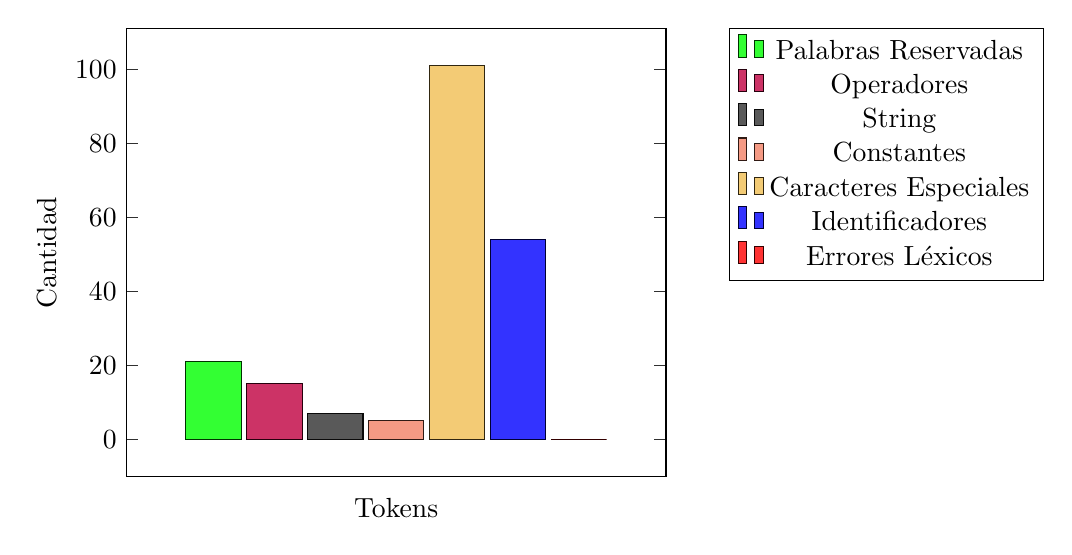
\begin{tikzpicture}
			\begin{axis}[
				ylabel=Cantidad,
				xlabel=Tokens,
				legend style={at={(1.7,1)}},
				bar width=20pt,
				ybar,
				xtick=\empty,
			]
			\addplot[green!20!black,fill=green!80!white]
				coordinates {(1,21)};
			\addplot[purple!20!black,fill=purple!80!white]
				coordinates {(1,15)};
			\addplot[gray!20!black,fill=gray!80!white]
				coordinates {(1,7)};
			\addplot[orange!20!black,fill=orange!80!white]
				coordinates {(1,5)};
			\addplot[yellow!20!black,fill=yellow!80!white]
				coordinates {(1,101)};
			\addplot[blue!20!black,fill=blue!80!white]
				coordinates {(1,54)};
			\addplot[red!20!black,fill=red!80!white]
				coordinates {(1,0)};
			\legend{\textcolor{black}{Palabras Reservadas},\textcolor{black}{Operadores},\textcolor{black}{String},\textcolor{black}{Constantes},\textcolor{black}{Caracteres Especiales},\textcolor{black}{Identificadores},\textcolor{black}{Errores Léxicos}}
			\end{axis}
		\end{tikzpicture}
	\end{frame}

    \section{}
    \begin{frame}{}
        \centering
            \Huge\bfseries
        \textcolor{orange}{The End}
    \end{frame}
\end{document}
